\chapter{Specifikacija programske potpore}
		
	\section{Funkcionalni zahtjevi}
			
			
			\noindent \textbf{Dionici:}
			
			\begin{packed_enum}
				
				\item Zaposlenik
				\item Revizor				
				\item Računovođa
				\item Direktor
				
			\end{packed_enum}
			
			\noindent \textbf{Aktori i njihovi funkcionalni zahtjevi:}
			
			
			\begin{packed_enum}
				\item  \underbar{Zaposlenik (inicijator) može:}
				
				\begin{packed_enum}
					
					\item skenirati dokument OCR-om
					\item vidjeti vlastitu povijest skeniranja
					\item poslati skenirani dokument revizoru ako je točno skeniran
					
				\end{packed_enum}
			
				\item  \underbar{Revizor (inicijator) može:}
				
				\begin{packed_enum}
					
					\item skenirati dokument OCR-om
					\item vidjeti vlastitu povijest skeniranja
					\item poslati skenirani dokument računovođama koji su za to namijenjeni
					
				\end{packed_enum}

                \item  \underbar{Računovođa (inicijator) može:}
				
				\begin{packed_enum}
					
					\item skenirati dokument OCR-om
					\item vidjeti vlastitu povijest skeniranja
					\item arhivirati dokumente ili ih poslati na potpisivanje direktoru
					\item primati direktorove obavijesti
					
				\end{packed_enum}

                \item  \underbar{Direktor (inicijator) može:}
				
				\begin{packed_enum}
					
					\item skenirati dokument OCR-om
					\item vidjeti vlastitu povijest skeniranja
					\item vidjeti povijest svih dokumenata svih korisnika
					\item vidjeti statistiku svih zaposlenika   
					\item primati računovođine obavijesti
					\item potpisivati dokumente
					
				\end{packed_enum}
			\end{packed_enum}
			
			\eject 
			
			
				
			\subsection{Obrasci uporabe}
				
				\subsubsection{Opis obrazaca uporabe}
					

					\noindent \underbar{\textbf{UC1 - Registracija}}
					\begin{packed_item}
	
						\item \textbf{Glavni sudionik:} Zaposlenik, revizor, računovođa, direktor
						\item  \textbf{Cilj:} Stvaranje stalnog računa te pristup onim funkcionalnostima aplikacije koje su korisniku potrebne
						\item  \textbf{Sudionici:} - Baza podataka
						\item  \textbf{Preduvjet:} - 
						\item  \textbf{Opis osnovnog tijeka:}
						
						\item[] \begin{packed_enum}
	
							\item Korisnik upisuje potrebne identifikacijske podatke
							\item Korisnik odabire specijalizaciju iz ponuđene liste dostupnih specijalizacija
							\item Korisnik biva obaviješten o registraciji
						\end{packed_enum}
						
						\item  \textbf{Opis mogućih odstupanja:}
						
						\item[] \begin{packed_item}
	
							\item[1.a]Korisnik upisuje podatke u neispravnom formatu 
							\item[] \begin{packed_enum}
								\item Sustav iznad krivo upisanog teksta navodi grešku
								\item Korisnik prepravlja unos prema uputama
							\end{packed_enum}
							\item[3.a]Korisnik je unio e-mail adresu koja već vezana za registriranog korisnika
							\item[] \begin{packed_enum}	
								\item Sustav obavještava korisnika o greški i vrača ga na ponovnu registraciju
								\item Korisnik unosi drugu e-mail adresu ili se prijavljuje sa zadnje unesenom
							\end{packed_enum}
						\end{packed_item}
					\end{packed_item}
					
					\noindent \underbar{\textbf{UC1.1: Odabir specijalizacije revizora}}
						\begin{packed_item}
		
							\item \textbf{Glavni sudionik:} Korisnik
							\item  \textbf{Cilj:} Odabir vrste dokumenta za kojeg će korisnik biti zadužen
							\item  \textbf{Sudionici:} - Baza podataka
							\item  \textbf{Preduvjet:} - Korisnik je na zaslonu registracije odabrao specijalizaciju računovođe
							\item  \textbf{Opis osnovnog tijeka:}
							
							\item[] \begin{packed_enum}
								\item Korisnik odabire za koji će tip dokumenta biti zadužen
							\end{packed_enum}
						\end{packed_item}

					\noindent \underbar{\textbf{UC2 - Prijava}}
						\begin{packed_item}
		
							\item \textbf{Glavni sudionik:} Zaposlenik, revizor, računovođa, direktor
							\item  \textbf{Cilj:} Prijava u sustav i početak korištenja usluga aplikacije
							\item  \textbf{Sudionici:} - Baza podataka
							\item  \textbf{Preduvjet:} - Korisnik je registriran
							\item  \textbf{Opis osnovnog tijeka:}
							
							\item[] \begin{packed_enum}
								\item Korisnik upisuje potrebne identifikacijske podatke
								\item Korisnik je preusmjeren na početni zaslon aplikacije
							\end{packed_enum}
							
							\item  \textbf{Opis mogućih odstupanja:}
							
							\item[] \begin{packed_item}
		
								\item[1.a]Korisnik upisuje neispravne podatke 
								\item[] \begin{packed_enum}
									\item Sustav u obliku pop-up teksta ispisuje poruku o neispravno unesenim podacima
									\item Korisnik prepravlja lozinku ili e-mail adresu
								\end{packed_enum}
							\end{packed_item}
						\end{packed_item}

					\noindent \underbar{\textbf{UC3 -  Odjava}}
						\begin{packed_item}
		
							\item \textbf{Glavni sudionik:} Zaposlenik, revizor, računovođa, direktor
							\item  \textbf{Cilj:} Odjava iz aplikacije u slučaju prijave drugog korisnika
							\item  \textbf{Sudionici:} - Baza podataka
							\item  \textbf{Preduvjet:} - Korisnik je prijavljen
							\item  \textbf{Opis osnovnog tijeka:}
							
							\item[] \begin{packed_enum}
								\item Korisnik odabire opciju "user info" na glavnom izborniku
								\item Korisnik se odjavljuje pritiskom na gumb za odjavu iz aplikacije
								\item Korisnik biva preusmjeren na zaslon aplikacije za prijavu
							\end{packed_enum}
						\end{packed_item}

					\noindent \underbar{\textbf{UC4 -  Skeniranje dokumenta}}
						\begin{packed_item}
		
							\item \textbf{Glavni sudionik:} Zaposlenik, revizor, računovođa, direktor
							\item  \textbf{Cilj:} Ispravno skenirati dokument te ga pohraniti u bazu podataka i u ovisnosti o specijalizaciji proslijediti ga drugom korisniku
							\item  \textbf{Sudionici:} - Baza podataka
							\item  \textbf{Preduvjet:} - Korisnik ima kameru na mobilnom uređaju
							\item  \textbf{Opis osnovnog tijeka:}
							
							\item[] \begin{packed_enum}
								\item Korisnik na glavnom izborniku odabire opciju "Scan"
								\item Korisnik uređaj pozicionira u skladu s dokumentom
								\item Korisnik čeka izvjesno vrijeme dok se uređaj ne stabilizira
								\item Korisnik pritiska gumb za okidanje slike
								\item Korisnik nakon provedenog OCR algoritma potvrđuje ispravnost skeniranja
								\item Korisnik o ovisnosti o specijalizaciji šalje dokument drugom korisniku ili ga arhivira
								\item Korisnik biva preusmjeren na zaslon spreman za ponovno skeniranje
							\end{packed_enum}
							
							\item  \textbf{Opis mogućih odstupanja:}
							
							\item[] \begin{packed_item}
		
								\item[1.a]Korisnik nema kameru na mobilnom uređaju 
								\item[] \begin{packed_enum}
									\item Na zaslonu se ispisuje poruka o nemogućnosti korištenja usluge skeniranja
								\end{packed_enum}
								\item[6.a]Korisnik nije zadovoljan skeniranim dokumentom
								\item[] \begin{packed_enum}
									\item Korisnik odabire opciju odbacivanja skeniranog dokumenta
									\item Korisnik ponovno skenira dokument
								\end{packed_enum}
							\end{packed_item}
						\end{packed_item}

					\noindent \underbar{\textbf{UC5 -  Pregled dokumenata}}
						\begin{packed_item}
		
							\item \textbf{Glavni sudionik:} Zaposlenik, revizor, računovođa, direktor
							\item  \textbf{Cilj:} Pregled onih dokumenata za koje je određeni korisnik odgovoran
							\item  \textbf{Sudionici:} - Baza podataka
							\item  \textbf{Preduvjet:} - Korisnik je prijavljen u sustav
							\item  \textbf{Opis osnovnog tijeka:}
							
							\item[] \begin{packed_enum}
								\item Korisnik na glavnom izborniku odabire opciju "History"
								\item Korisnik na temelju specijalizacije odabire opcije prikaza dokumenata
								\item Korisniku se prikazuju dokumenti
							\end{packed_enum}
							
							\item  \textbf{Opis mogućih odstupanja:}
							
							\item[] \begin{packed_item}
		
								\item[3.a]Korisnik za odabranu opciju nema dostupnih dokumenata
								\item[] \begin{packed_enum}
									\item Na zaslonu se umjesto popisa dokumenata ispsuje poruka
								\end{packed_enum}
							\end{packed_item}
						\end{packed_item}

					\noindent \underbar{\textbf{UC5.1 -  Pregled svih dokumenata}}
						\begin{packed_item}
		
							\item \textbf{Glavni sudionik:} Direktor
							\item  \textbf{Cilj:} Pregled svih skeniranih dokumenata svih korisnika
							\item  \textbf{Sudionici:} - Baza podataka
							\item  \textbf{Preduvjet:} - Korisnik je prijavljen u sustav i ima nivo autorizacije direktora
							\item  \textbf{Opis osnovnog tijeka:}
							
							\item[] \begin{packed_enum}
								\item Korisnik na glavnom izborniku odabire opciju "History"
								\item Korisnik iz izbornika filtera odabire opciju prikaza svih dokumenata
								\item Korisniku se prikazuju svi dokumenti svih korisnika
							\end{packed_enum}
							
							\item  \textbf{Opis mogućih odstupanja:}
							
							\item[] \begin{packed_item}
		
								\item[3.a]Korisnik za odabranu opciju nema dostupnih dokumenata
								\item[] \begin{packed_enum}
									\item Na zaslonu se umjesto popisa dokumenata ispsuje poruka
								\end{packed_enum}
							\end{packed_item}
						\end{packed_item}

					\noindent \underbar{\textbf{UC5.2 -  Pregled dokumenata za potpisivanje}}
						\begin{packed_item}
		
							\item \textbf{Glavni sudionik:} Direktor
							\item  \textbf{Cilj:} Pregled i potpisivanje dokumenata koje je prije arhiviranja potrebno potpisati
							\item  \textbf{Sudionici:} - Baza podataka
							\item  \textbf{Preduvjet:} - Korisnik je prijavljen u sustav i ima nivo autorizacije direktora
							\item  \textbf{Opis osnovnog tijeka:}
							
							\item[] \begin{packed_enum}
								\item Korisnik na glavnom izborniku odabire opciju "History"
								\item Korisnik iz izbornika filtera odabire opciju prikaza dokumenata za potpisivanje
								\item Korisniku se prikazuju svi dokumenti koji su spremni za potpisivanje
							\end{packed_enum}
							
							\item  \textbf{Opis mogućih odstupanja:}
							
							\item[] \begin{packed_item}
		
								\item[3.a]Korisnik za odabranu opciju nema dostupnih dokumenata
								\item[] \begin{packed_enum}
									\item Na zaslonu se umjesto popisa dokumenata ispsuje poruka
								\end{packed_enum}
							\end{packed_item}
						\end{packed_item}

					\noindent \underbar{\textbf{UC5.3 -  Pregled dokumenata za arhiviranje}}
						\begin{packed_item}
		
							\item \textbf{Glavni sudionik:} Računovođa
							\item  \textbf{Cilj:} Pregled svih dokumenata spremnih za arhiviranje
							\item  \textbf{Sudionici:} - Baza podataka
							\item  \textbf{Preduvjet:} - Korisnik je prijavljen u sustav i ima nivo autorizacije računovođe
							\item  \textbf{Opis osnovnog tijeka:}
							
							\item[] \begin{packed_enum}
								\item Korisnik na glavnom izborniku odabire opciju "History"
								\item Korisnik iz izbornika filtera odabire opciju prikaza dokumenata spremnih za arhiviranje
								\item Korisniku se prikazuju svi dokumenti spremni za arhiviranje
							\end{packed_enum}
							
							\item  \textbf{Opis mogućih odstupanja:}
							
							\item[] \begin{packed_item}
		
								\item[3.a]Korisnik za odabranu opciju nema dostupnih dokumenata
								\item[] \begin{packed_enum}
									\item Na zaslonu se umjesto popisa dokumenata ispsuje poruka
								\end{packed_enum}
							\end{packed_item}
						\end{packed_item}

					\noindent \underbar{\textbf{UC5.4 -  Pregled dokumenata za reviziju}}
						\begin{packed_item}
		
							\item \textbf{Glavni sudionik:} Revizor
							\item  \textbf{Cilj:} Pregled dokumenata spremnih za reviziju
							\item  \textbf{Sudionici:} - Baza podataka
							\item  \textbf{Preduvjet:} - Korisnik je prijavljen u sustav i ima nivo autorizacije revizora
							\item  \textbf{Opis osnovnog tijeka:}
							
							\item[] \begin{packed_enum}
								\item Korisnik na glavnom izborniku odabire opciju "History"
								\item Korisnik iz izbornika filtera odabire opciju prikaza dokumenata spremnih za reviziju
								\item Korisniku se prikazuju svi dokumenti svih korisnika
							\end{packed_enum}
							
							\item  \textbf{Opis mogućih odstupanja:}
							
							\item[] \begin{packed_item}
		
								\item[3.a]Korisnik za odabranu opciju nema dostupnih dokumenata
								\item[] \begin{packed_enum}
									\item Na zaslonu se umjesto popisa dokumenata ispsuje poruka
								\end{packed_enum}
							\end{packed_item}
						\end{packed_item}

					\noindent \underbar{\textbf{UC5.5 -  Pregled vlastito skeniranih dokumenata}}
						\begin{packed_item}
		
							\item \textbf{Glavni sudionik:} Zaposlenik, revizor, računovođa, direktor
							\item  \textbf{Cilj:} Pregled svih dokumenata koje je skenirao trenutno prijavljeni korisnik
							\item  \textbf{Sudionici:} - Baza podataka
							\item  \textbf{Preduvjet:} - Korisnik je prijavljen u sustav
							\item  \textbf{Opis osnovnog tijeka:}
							
							\item[] \begin{packed_enum}
								\item Korisnik na glavnom izborniku odabire opciju "History"
								\item Korisnik iz izbornika filtera odabire opciju prikaza svih vlastito skeniranih
								\item Korisniku se prikazuju svi dokumenti svih korisnika
							\end{packed_enum}
							
							\item  \textbf{Opis mogućih odstupanja:}
							
							\item[] \begin{packed_item}
		
								\item[3.a]Korisnik za odabranu opciju nema dostupnih dokumenata
								\item[] \begin{packed_enum}
									\item Na zaslonu se umjesto popisa dokumenata ispsuje poruka
								\end{packed_enum}
							\end{packed_item}
						\end{packed_item}

					\noindent \underbar{\textbf{UC6 - Pregled korisničkih podataka}}
						\begin{packed_item}
		
							\item \textbf{Glavni sudionik:} Zaposlenik, revizor, računovođa, direktor
							\item  \textbf{Cilj:} Pregled korisničkih podataka vezanih za trenutno prijavljenog korisnika
							\item  \textbf{Sudionici:} - Baza podataka
							\item  \textbf{Preduvjet:} - Korisnik je prijavljen u sustav
							\item  \textbf{Opis osnovnog tijeka:}
							
							\item[] \begin{packed_enum}
								\item Korisnik na glavnom izborniku odabire opciju "Info"
								\item Korisniku se prikazuju korisnički podaci
							\end{packed_enum}
						\end{packed_item}

					\noindent \underbar{\textbf{UC7 - Slanje dokumenta revizoru}}
						\begin{packed_item}
		
							\item \textbf{Glavni sudionik:} Zaposlenik
							\item  \textbf{Cilj:} Slanje skeniranog dokumenta odgovarajućem korisniku u svrhu daljnje obrade
							\item  \textbf{Sudionici:} - Baza podataka
							\item  \textbf{Preduvjet:} - Korisnik je prijavljen u sustav i ima nivo autorizacije zaposlenika
							\item  \textbf{Opis osnovnog tijeka:}
							
							\item[] \begin{packed_enum}
								\item Korisnik na glavnom izborniku odabire opciju "scan"
								\item Korisnik skenira dokument
								\item Korisniku potvrđuje kvalitetu skeniranog dokumenta
								\item Korisnik šalje dokument revizoru
							\end{packed_enum}
						\end{packed_item}

					\noindent \underbar{\textbf{UC8 - Slanje dokumenta računovođi}}
						\begin{packed_item}
		
							\item \textbf{Glavni sudionik:} Revizor
							\item  \textbf{Cilj:} Slanje dokumenta računovođama koji su zaduženi za određeni tip skeniranog dokumenta
							\item  \textbf{Sudionici:} - Baza podataka
							\item  \textbf{Preduvjet:} - Korisnik je prijavljen i ima nivo autorizacije revizora
							\item  \textbf{Opis osnovnog tijeka:}
							
							\item[] \begin{packed_enum}
								\item Korisnik prilikom pregleda dokumenata odabire dokument spreman za reviziju
								\item Korisnik odabire tip dokumenta kako bi dokument bio proslijeđen ispravnim računovođama
							\end{packed_enum}
							
							\item  \textbf{Opis mogućih odstupanja:}
							
							\item[] \begin{packed_item}
		
								\item[1.a]Korisnik kod pregleda dokumenata za odabranu opciju nema dostupnih dokumenata
								\item[] \begin{packed_enum}
									\item Na zaslonu se umjesto popisa dokumenata ispsuje poruka
								\end{packed_enum}
							\end{packed_item}

							\item  \textbf{Alternativni tijek:}

							\item[] \begin{packed_item}
		
								\item[1.a]Korisnik skenira dokument
								\item[2.a]Ako je korisnik skenirao dokument, aplikacija sama prepoznaje tip dokumenta
							\end{packed_item}
						\end{packed_item}
					\noindent \underbar{\textbf{UC9 - Arhiviranje dokumenata}}
						\begin{packed_item}
		
							\item \textbf{Glavni sudionik:} Računovođa
							\item  \textbf{Cilj:} Spremanje potpuno obrađenih dokumenata u bazu podataka
							\item  \textbf{Sudionici:} - Baza podataka
							\item  \textbf{Preduvjet:} - Korisnik je prijavljen u sustav i ima nivo autorizacije računovođe
							\item  \textbf{Opis osnovnog tijeka:}
							
							\item[] \begin{packed_enum}
								\item Korisnik odabire pregled dokumenata
								\item Korisnik odabire opciju prikaza dokumenata dostupnih za arhiviranje
								\item Korisnik odabire dokument koji želi arhivirati
								\item Korisnik arhivira zadani dokument
							\end{packed_enum}
							
							\item  \textbf{Alternativni tijek:}

							\item[] \begin{packed_item}
		
								\item[1-3.a]Korisnik dobiva obavijest
								\item[] \begin{packed_enum}
									\item Korisnik pritiskom na obavijest dolazi do zaslona na kojem se prikazuje dokument
								\end{packed_enum}
							\end{packed_item}
						\end{packed_item}

					\noindent \underbar{\textbf{UC10 - Slanje dokumenta na potpis}}
						\begin{packed_item}
		
							\item \textbf{Glavni sudionik:} Računovođa
							\item  \textbf{Cilj:} Pregled svih skeniranih dokumenata svih korisnika
							\item  \textbf{Sudionici:} - Baza podataka
							\item  \textbf{Preduvjet:} - Korisnik je prijavljen u sustav i ima nivo autorizacije računovođe
							\item  \textbf{Opis osnovnog tijeka:}
							
							\item[] \begin{packed_enum}
								\item Korisnik odabire opciju "History"
								\item Korisnik iz izbornika filtera odabire opciju prikaza dokumenata za potpis
								\item Korisnik odabire dokument koji želi poslati na potpis
								\item korisnik šalje dokument na potpis
							\end{packed_enum}

							\item  \textbf{Alternativni tijek:}

							\item[] \begin{packed_item}
		
								\item[1-3.a]Korisnik skenira dokument
								\item[] \begin{packed_enum}
									\item Korisnik odabire opciju "Scan"
									\item Korisnik skenira dokument
									\item Korisnik potvrđuje kvalitetu skeniranog dokumenta
									\item Korisnik odabire opciju slanja dokumenta na potpis
								\end{packed_enum}
								\item  \textbf{Opis mogućih odstupanja:}
							
								\item[] \begin{packed_item}
			
									\item[4.]Korisnik odabire opciju arhiviranja dokumenta
									\item[] \begin{packed_enum}
										\item Korisnik biva prebačen na zaslon skeniranja
									\end{packed_enum}
								\end{packed_item}
							\end{packed_item}
						\end{packed_item}

					\noindent \underbar{\textbf{UC11 - Primanje obavijesti}}
						\begin{packed_item}
		
							\item \textbf{Glavni sudionik:} Direktor, računovođa
							\item  \textbf{Cilj:} Brzi pristup dokumentu kojega je potrebno obraditi
							\item  \textbf{Sudionici:} - Baza podataka
							\item  \textbf{Preduvjet:} - Korisniku je poslan dokument od strane drugog korisnika
							\item  \textbf{Opis osnovnog tijeka:}
							
							\item[] \begin{packed_enum}
								\item Korisnik otvara obavijest
								\item Korisnik biva preusmjeren na zaslon koji sadrži podatke o dokumentu
								\item Korisnik obrađuje dokument na način na koji je za to zadužen
							\end{packed_enum}
							
							\item  \textbf{Opis mogućih odstupanja:}
							
							\item[] \begin{packed_item}
		
								\item[1.a]Korisnik briše obavijest
								\item[] \begin{packed_enum}
									\item Korisnik nastavlja rad, a dokument se obrađuje klikom na određeni dokument na zaslonu pregleda dokumenata
								\end{packed_enum}
							\end{packed_item}
						\end{packed_item}

					\noindent \underbar{\textbf{UC12 - Potpisivanje dokumenta}}
						\begin{packed_item}
		
							\item \textbf{Glavni sudionik:} Direktor
							\item  \textbf{Cilj:} Označavanje dokumenta potpisanim
							\item  \textbf{Sudionici:} - Baza podataka
							\item  \textbf{Preduvjet:} - Korisnik je prijavljen u sustav i ima nivo autorizacije direktora
							\item  \textbf{Opis osnovnog tijeka:}
							
							\item[] \begin{packed_enum}
								\item Korisnik na glavnom izborniku odabire opciju "History"
								\item Korisnik iz izbornika filtera odabire opciju prikaza dokumenata za potpisivanje
								\item Korisniku se prikazuju svi dokumenti za potpisivanje
								\item Korisnik odabire dokument koji želi potpisati
								\item Korisniku se prikazuju podaci odabranog dokumenta
								\item Korisnik potpisuje dokument
							\end{packed_enum}
							
							\item  \textbf{Opis mogućih odstupanja:}
							
							\item[] \begin{packed_item}
		
								\item[4.a]Dokument je već potpisan od strane drugog računovođe
								\item[] \begin{packed_enum}
									\item Korisnik nastavlja rad
								\end{packed_enum}
							\end{packed_item}

							\item  \textbf{Alternativni koraci:}

							\item[] \begin{packed_item}
		
								\item[1-4.a]Korisnik je dobio obavijest
								\item[] \begin{packed_enum}
									\item Korisnik pritišće na obavijest
									\item Korisniku se prikazuju podaci dokumenta referenciranog u obavijesti
								\end{packed_enum}
							\end{packed_item}
						\end{packed_item}

					\noindent \underbar{\textbf{UC13 - Pregled statistike}}
						\begin{packed_item}
		
							\item \textbf{Glavni sudionik:} Direktor
							\item  \textbf{Cilj:} Uvid u statistiku zaposlenika
							\item  \textbf{Sudionici:} - Baza podataka
							\item  \textbf{Preduvjet:} - Korisnik je prijavljen u sustav i ima nivo autorizacije direktora
							\item  \textbf{Opis osnovnog tijeka:}
							
							\item[] \begin{packed_enum}
								\item Korisnik na glavnom izborniku odabire opciju "Info"
								\item Korisnik odabire opciju "Statistics"
								\item Korisniku se prikazuje lista svih zaposlenika
								\item Korisnik odabire zaposlenika za kojega želi prikazati statistiku
								\item Korisniku se prikazuje zaslon s odgovarajućom statistikom
							\end{packed_enum}
						\end{packed_item}
				\subsubsection{Dijagrami obrazaca uporabe}
				
				
				%unos slike
				\begin{figure}[H]
					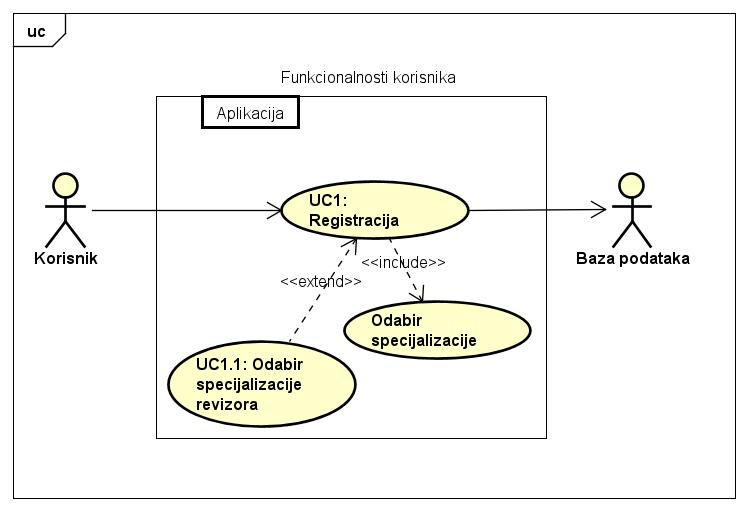
\includegraphics[scale=0.5]{slike/Funkcionalnosti korisnika} %veličina slike u odnosu na originalnu datoteku i pozicija slike
					\centering
					\caption{ Dijagram obrasca uporabe, funkcionalnosti korisnika}
					\label{fig:promjene}
				\end{figure}

				%unos slike
				\begin{figure}[H]
					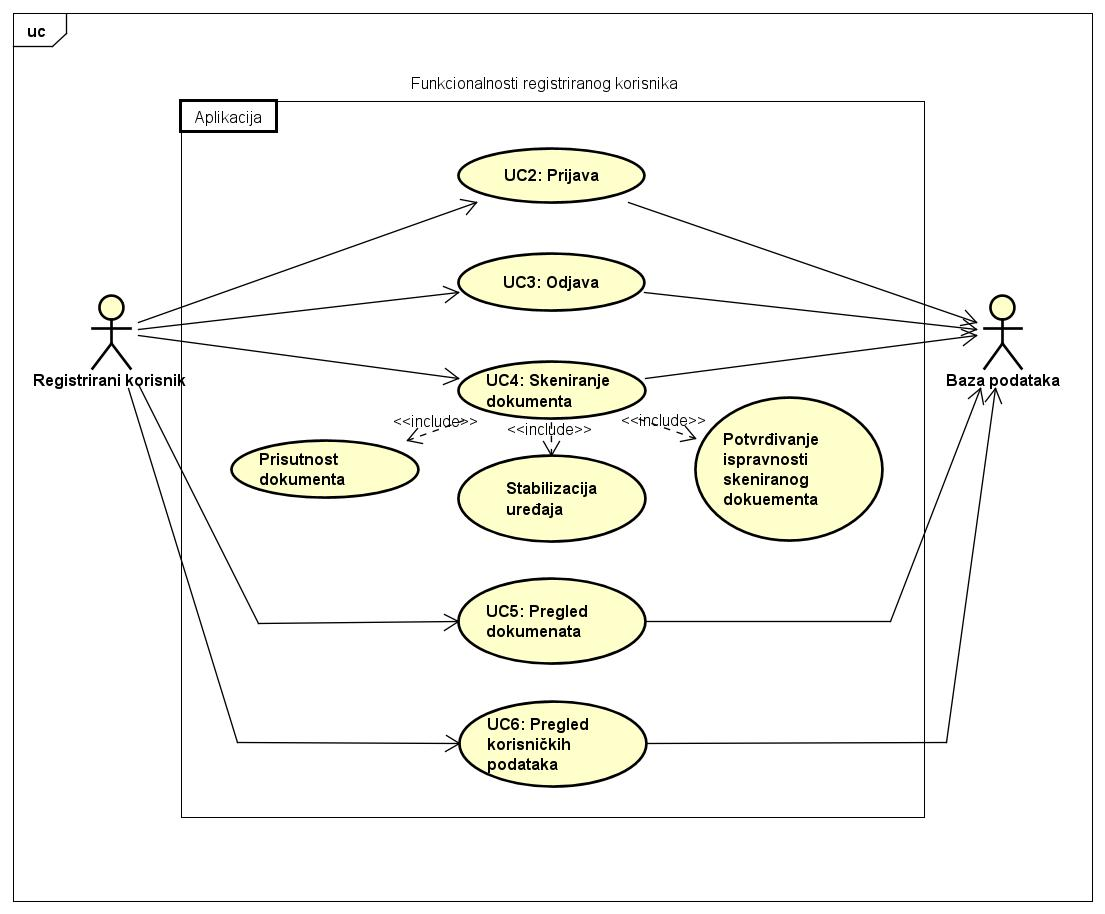
\includegraphics[scale=0.4]{slike/Funkcionalnosti registriranog korisnika} %veličina slike u odnosu na originalnu datoteku i pozicija slike
					\centering
					\caption{ Dijagram obrasca uporabe, funkcionalnosti registriranog korisnika}
					\label{fig:promjene}
				\end{figure}

				%unos slike
				\begin{figure}[H]
					\includegraphics[scale=0.4]{slike/funkcionalnosti specijalizacija} %veličina slike u odnosu na originalnu datoteku i pozicija slike
					\centering
					\caption{ Dijagram obrasca uporabe, funkcionalnosti specijalizacija}
					\label{fig:promjene}
				\end{figure}

				%unos slike
				\begin{figure}[H]
					\includegraphics[scale=0.3]{slike/pregled dokumenata} %veličina slike u odnosu na originalnu datoteku i pozicija slike
					\centering
					\caption{ Dijagram obrasca uporabe, pregled dokumenata}
					\label{fig:promjene}
				\end{figure}
				\eject		
				
			\subsection{Sekvencijski dijagrami}


				\subsubsection{Obrazac uporabe UC1 - Registracija}
				Korisnik otvara aplikaciju te mu aplikacija u slučaju da nitko na uređaju nije prijavljen u sustav prikazuje zaslon za registraciju novog korisnika. Dok korisnik unosi identifikacijske podatke aplikacija konstantno provjerava ispravnost formata unesenih podataka kao što je dovoljno jaka lozinka ili ispravan format e-mail adrese te u slučaju detektiranja greške ispisuje odgovarajuću poruku iznad polja u kojem je greška. Nakon što korisnik unese podatke ispravnog formata, pritišće gumb za registraciju. Ako se je korisnik specijalizirao kao računovođa, aplikacija mu ispisuje izbornik sa svim tipovima dokumenata koji su dostupni. Korisnik odabire dokument za koji će biti zadužen te potvrđuje odabir. Aplikacija unesene podatke šalje u bazu podataka gdje se podaci provjeravaju. Ako baza podataka ustanovi da korisnik s istom e-mail adresom već postoji, registracija se odbacuje i korisniku se ispisuje odgovarajuća poruka. Ako je registracija uspjela, korisnik biva preusmjeren na početni zaslon aplikacije.
				%unos slike
				\begin{figure}[H]
					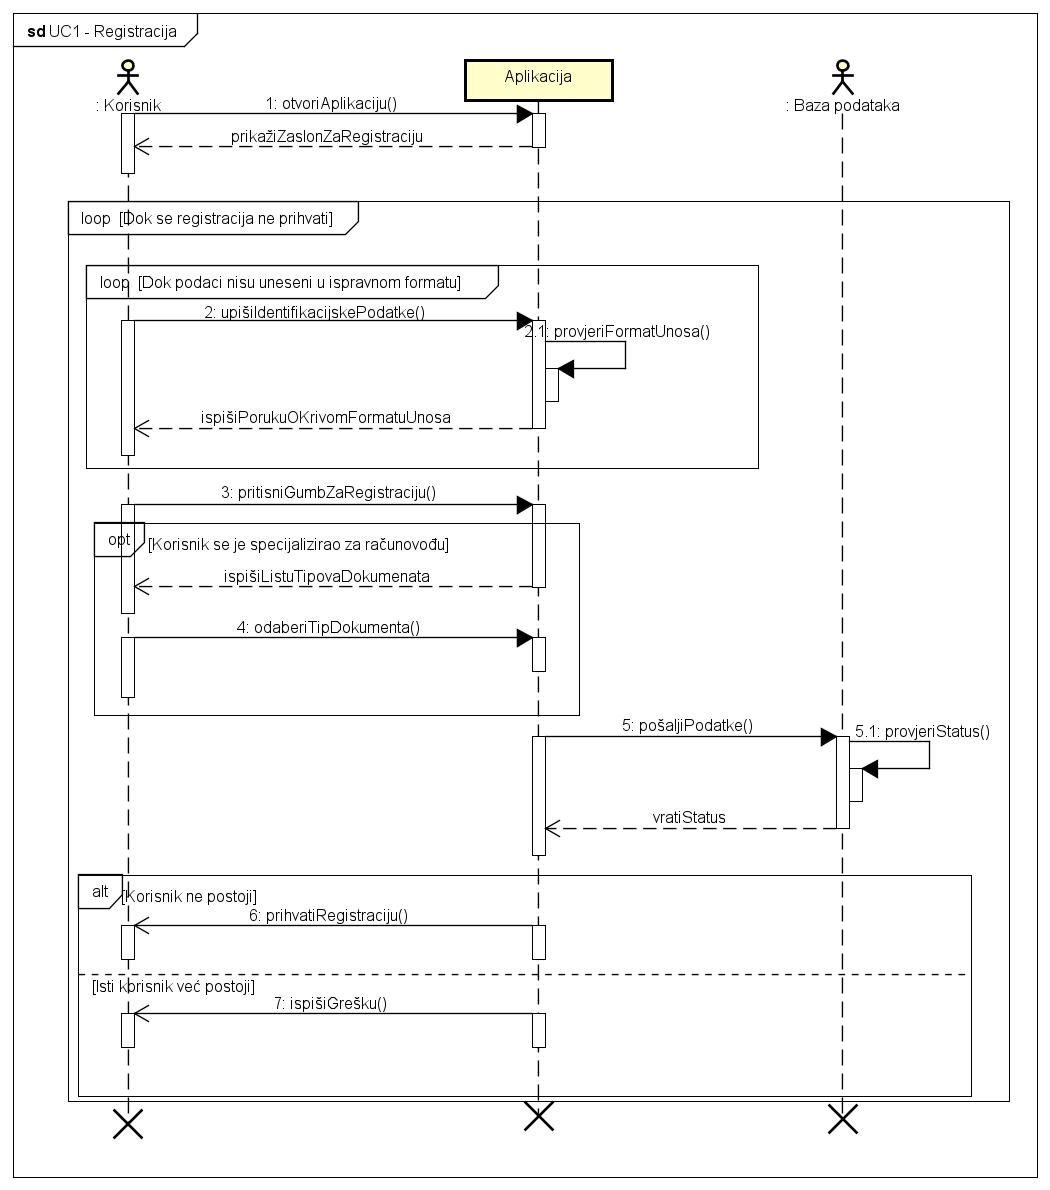
\includegraphics[scale=0.35]{slike/UC1 - Registracija} %veličina slike u odnosu na originalnu datoteku i pozicija slike
					\centering
					\caption{ Sekvencijalni dijagram, UC1}
					\label{fig:promjene}
				\end{figure}

				\subsubsection{Obrazac uporabe UC4 - Skeniranje}
				Korisnik na glavnom izborniku odabire opciju skeniranja te mu aplikacija na zaslonu prikazuje pogled kamere. Aplikacija korisniku ne dozvoljava skeniranje prije nego što su zadovoljena dva uvjeta. Prvi uvjet je da se u pogledu kamere nalazi dokument. Drugi uvjet je ispunjen kada aplikacija u određenom periodu vremena ne izmjeri vibracije sa senzora na mobilnom uređaju. Kada je dokument prisutan i uređaj je stabilan, aplikacija korisniku omogućuje okidanje fotografije. Aplikacija nakon okidanja fotografije izvodi OCR algoritam. Nakon izvedenog algoritma aplikacija korisniku daje opciju prihvaćanja ili odbacivanja skeniranog dokumenta na temelju kvalitete skeniranja. Ako korisnik odbaci skenirani dokument, aplikacija dokument pohranjuje u bazu podataka s oznakom da je neispravno skeniran. Ako korisnik prihvati skenirani dokument, aplikacija u bazu podataka pohranjuje dokument s oznakom da je ispravno skeniran.
				%unos slike
				\begin{figure}[H]
					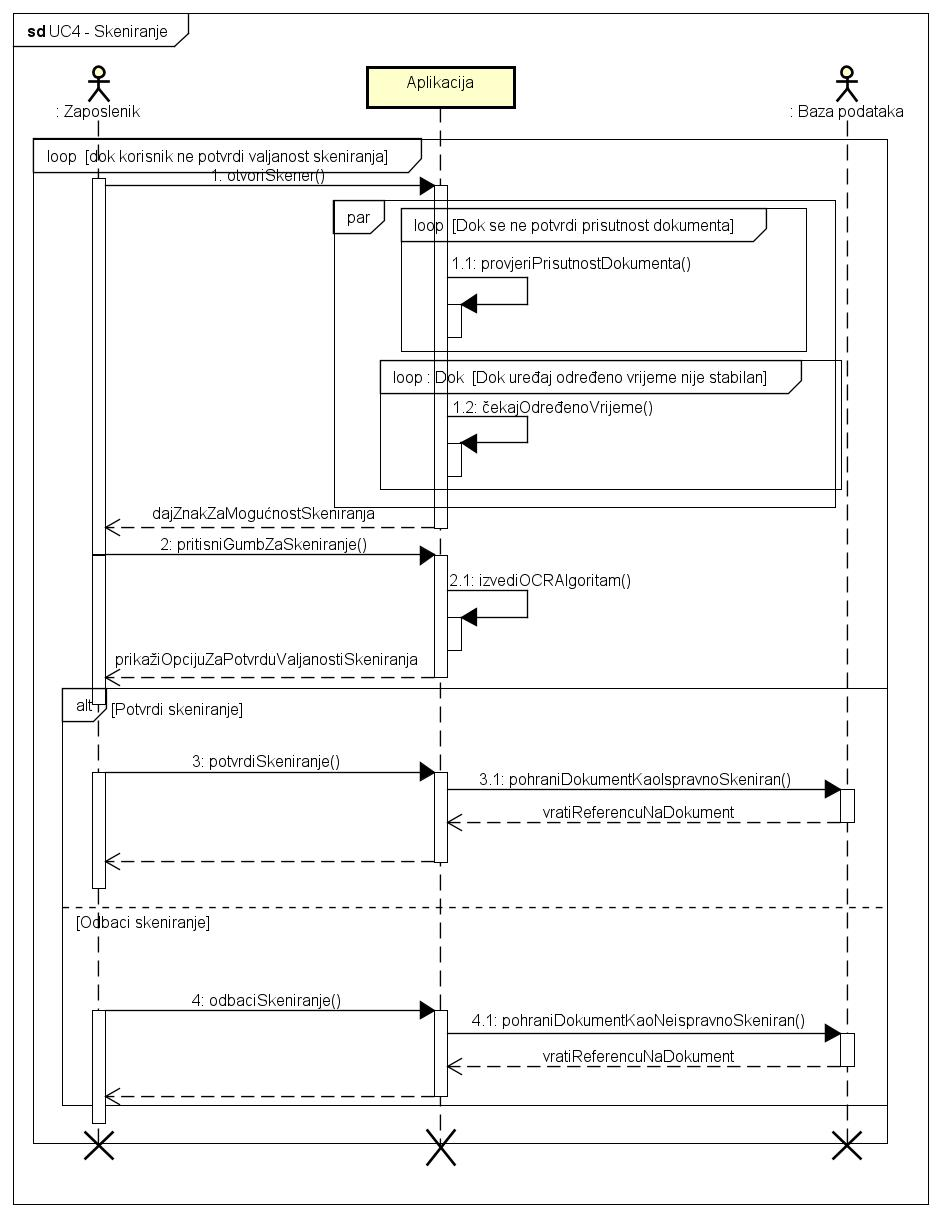
\includegraphics[scale=0.35]{slike/UC4 - Skeniranje} %veličina slike u odnosu na originalnu datoteku i pozicija slike
					\centering
					\caption{ Sekvencijalni dijagram, UC4}
					\label{fig:promjene}
				\end{figure}


				\subsubsection{Obrazac uporabe UC8 - Slanje dokumenta računovođi}
				Revizor dokument računovođi na arhiviranje može poslati na dva načina. U slučaju da računovođi treba poslati dokument koji je već skeniran od strane zaposlenika, revizor u pregledu dokumenata odabire filtar za prikaz dokumenata spremnih za slanje računovođi. Aplikacija iz baze podataka dohvaća tražene dokumente i prikazuje ih revizoru. Revizor na izborniku odabire željeni dokument. Aplikacija otvara izabrani dokument i prikazuje ga revizoru. Revizor odabire opciju slanja dokumenta računovođi. Budući da je svaki računovođa zadužen za određeni tip dokumenta, aplikacija revizoru prikazuje izbornik koji sadrži popis svih tipova dokumenta. Revizor izabire onaj tip dokumenta koji odgovara skeniranom dokumentu. Aplikacija u bazi podataka mijenja status dokumenta što dokument čini vidljivim računovođi. Revizor ponavlja radnju sve dok ne pošalje sve željene dokumente. \par U slučaju da revizor treba poslati dokument kojeg još nije skenirao zaposlenik, revizor treba skenirati dokument sam. Nakon skeniranja aplikacija dokumentu automatski odredi tip i pohrani ga u bazu podataka.
				%unos slike
				\begin{figure}[H]		
					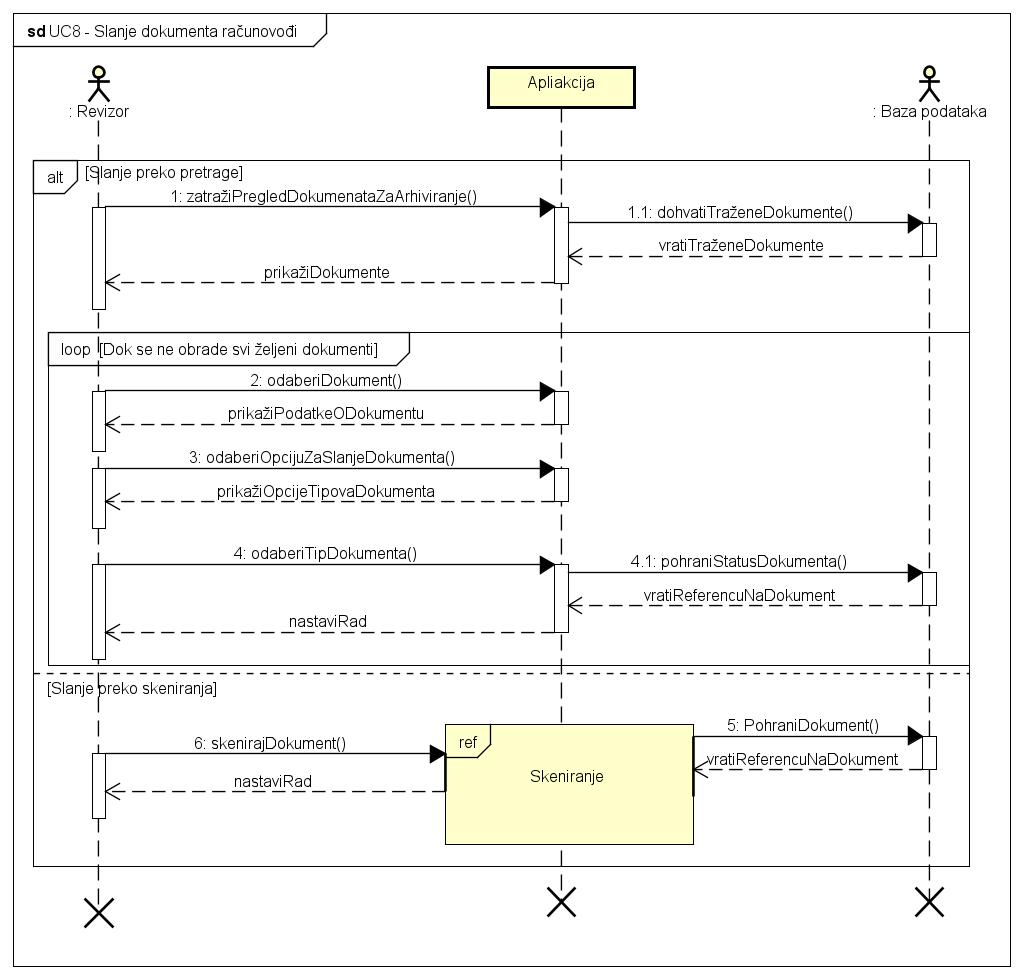
\includegraphics[scale=0.35]{slike/UC8 - Slanje dokumenta računovođi} %veličina slike u odnosu na originalnu datoteku i pozicija slike
					\centering
					\caption{ Sekvencijalni dijagram, UC8}
					\label{fig:promjene}
				\end{figure}

				\subsubsection{Obrazac uporabe UC12 - Potpisivanje dokumenata}
				Računovođa dokument može potpisati na dva načina. Jedan način je da direktor nakon što računovođa pošalje dokument na potpisivanje dobije obavijest. Aplikacija direktoru prikazuje obavijest na alatnoj traci mobilnog uređaja. Nakon što direktor otvara obavijest, aplikacija dohvaća dokument referenciran u obavijesti iz baze podataka i prikazuje ga na zaslonu. Direktor odabire opciju potpisivanja dokumenta. Aplikacija u bazu podataka pohrani potpis gdje se aktivira slanje obavijesti računovođi koji je zadužen za arhiviranje istog dokumenta. Direktor nastavlja rad. \par Drugi način je da direktor sam dolazi do dokumenta kojega treba potpisati. Direktor u pregledu povijesti dokumenata odabire filtar kojim od aplikacije zatraži prikaz samo onih dokumenata spremnih za potpisivanje. Aplikacija prikazuje tražene dokumente. Direktor odabire željeni dokument te ga potpisuje. Aplikacija potpis sprema u bazu podataka što uzrokuje slanje obavijesti računovođi koji je zadužen za arhiviranje istog dokumenta. Direktor ponavlja radnje sve dok ne završi s potpisivanjem svih željenih dokumenata.
				%unos slike
				\begin{figure}[H]
					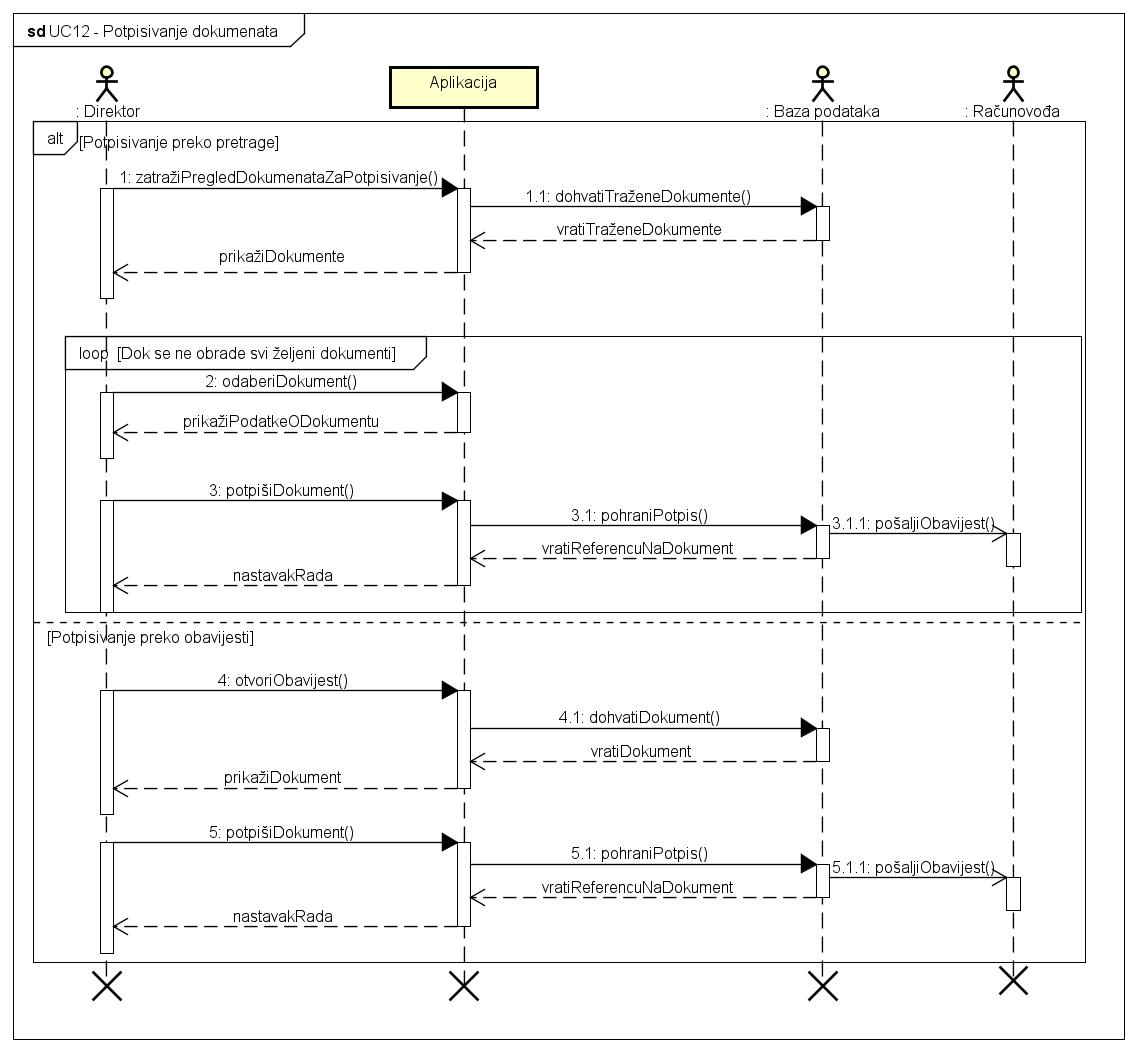
\includegraphics[scale=0.35]{slike/UC12 - Potpisivanje dokumenata} %veličina slike u odnosu na originalnu datoteku i pozicija slike
					\centering
					\caption{ Sekvencijalni dijagram, UC12}
					\label{fig:promjene}
				\end{figure}
				\eject
	
		\section{Ostali zahtjevi}
		\begin{packed_item}
			\item{Aplikacija mora omogućiti primanje obavijesti i kada korisnik nema otvorenu instancu aplikacije}
			\item{Izvođenje OCR algoritma ne smije trajati duže od nekoliko sekundi}
			\item{Sustav mora podržavati rad od 50 do 100 korisnika u stvarnom vremenu}
			\item{Aplikacija za detektiranje prisutnosti dokumenta mora koristiti detekciju rubova}
			\item{Sustav za praćenje broja skeniranih dokumenata koristi pomoćnu strukturu podataka kako bi se smanjio broj upita u bazu podataka}
			\item{Sustav za prikaz velikog broja dokumenata mora koristi paginaciju \textit{(eng. pagination)}}
			\item{Aplikacija prilikom ponovnog otvaranja mora pamtiti zadnje prijavljenog korisnika}
			\item{Aplikacija prilikom pregleda dokumenata mora omogućiti naprednije filtriranje i sortiranje}
			\item{Aplikacija mora podržavati prijavu različitih korisnika na istom uređaju}
		\end{packed_item}
			
			 
			 
			 
	